% Chapter 4: Experimental Procedure 
\chapter{Appendices}
\label{chapter:appendices}

\graphicspath{ {report/Appendices/assets/} } 

% \setlength{\voffset}{0cm}
% \setlength{\hoffset}{0cm}

\section{EEG Hardware Schematics}

\label{appendix:schematics}
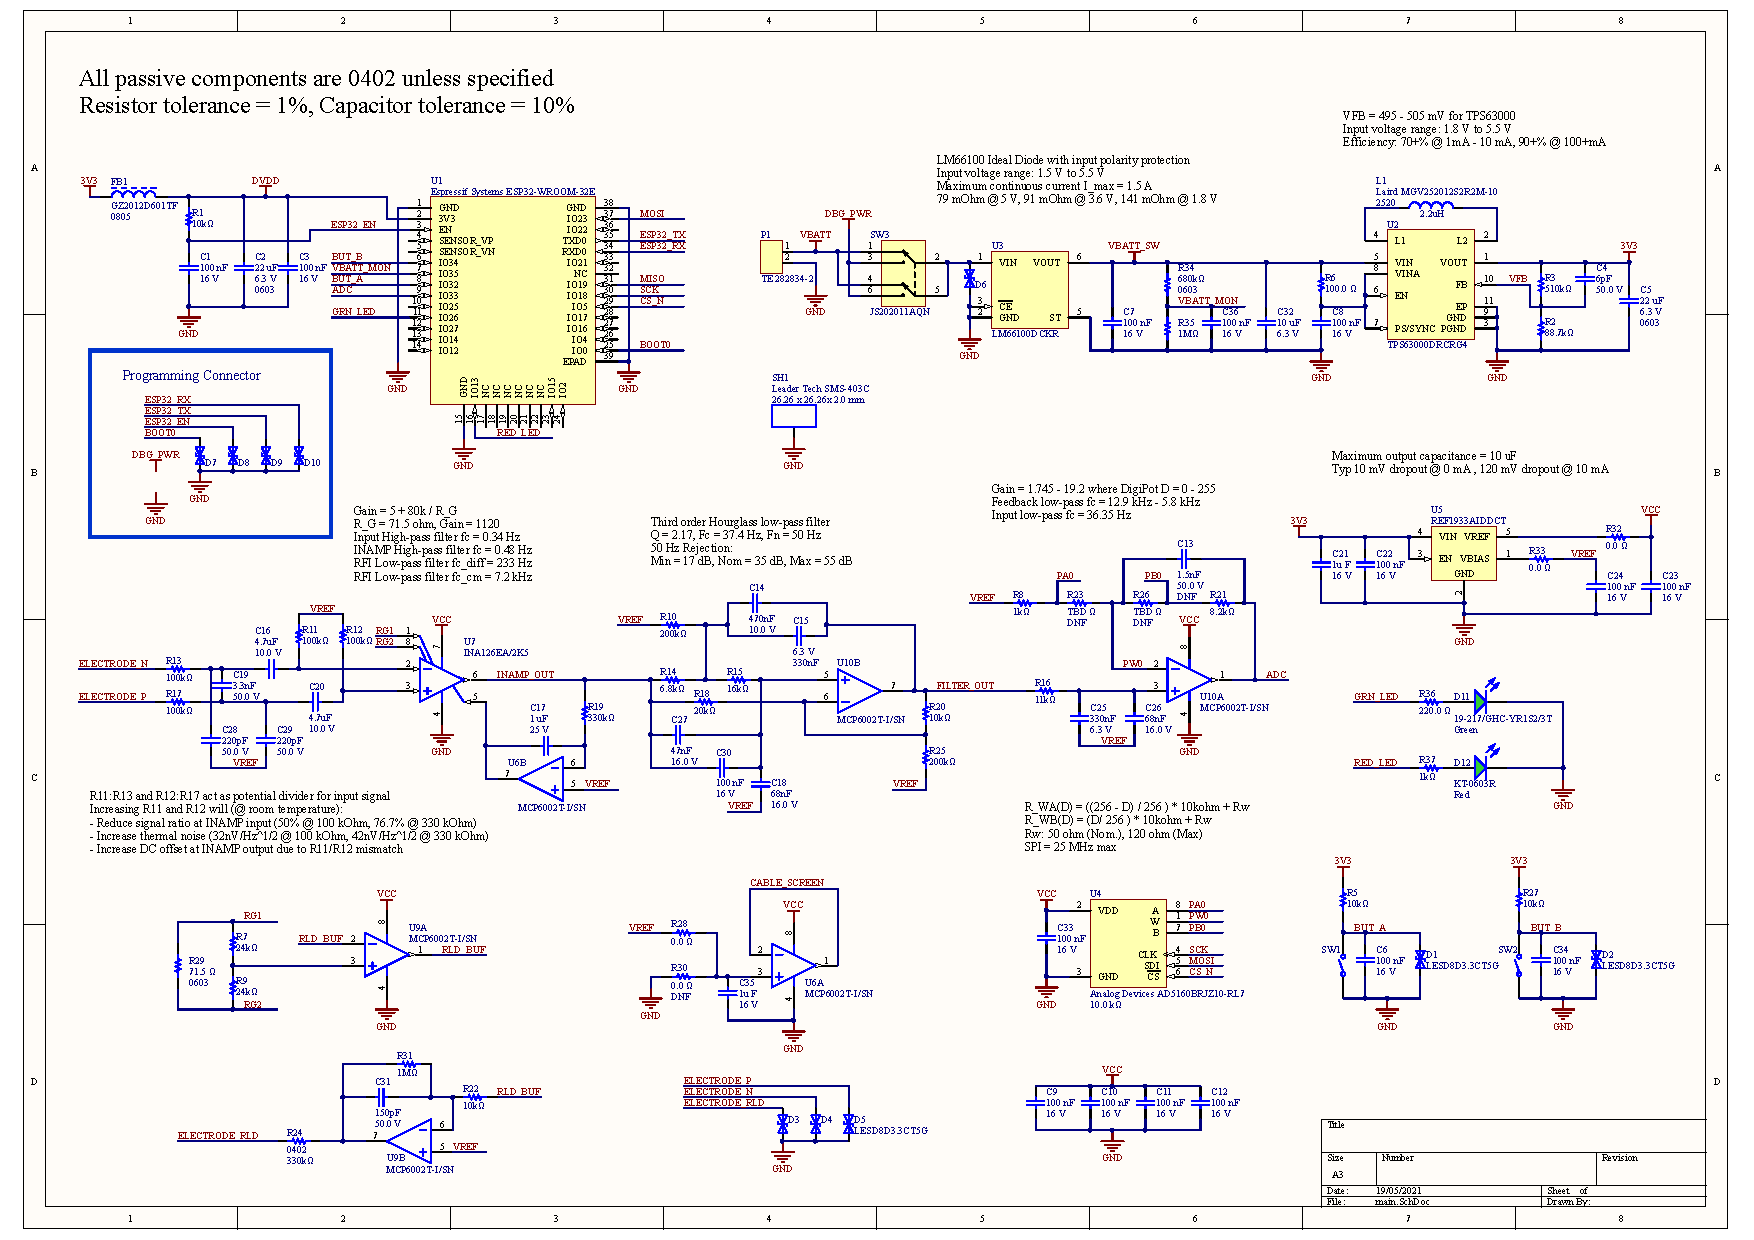
\includepdf[pages=-]{schematics.PDF}

\section{Firmware Implementations}
\label{app:firmware}

\begin{listing}[h]
\small
\begin{minted}{python}
from ulab import numpy as np

def power_iteration(A, iterations):
    """
    Iterative algo. to find the eigenvector of a matrix A corresponding to the largest
    eigenvalue.
    
    """
    # choose random initial vector to reduce risk of choosing one orthogonal to 
    # target eigen vector
    b_k = np.array([urandom.random() for i in range(len(A))])

    for _ in range(iterations):
        b_k1 = np.dot(A, b_k)
        b_k1_norm = np.linalg.norm(b_k1)
        # re normalize the vector
        b_k = b_k1 / b_k1_norm

    return b_k1_norm, b_k

\end{minted}
\caption{MicroPython implementation of power iteration algorithm for finding the maximum real eigenvalue of an arbitrary matrix \ref{algo:gen-eig-algo}}
\label{app-listing:power-iteration-mpy}
\end{listing}

\begin{listing}[h]
\small
\begin{minted}{python}
from ulab import numpy as np

def solve_gen_eig_prob(A, B, eps=1e-6):
    """
    Solves the generalised eigenvalue problem of the form:
    Aw = lambda*Bw
    
    Note: can be validated against `scipy.linalg.eig(A, b=B)`
    
    Ref: 
    'Eigenvalue and Generalized Eigenvalue Problems: Tutorial (2019)'
    Benyamin Ghojogh and Fakhri Karray and Mark Crowley
    arXiv 1903.11240

    """
    Lam_b, Phi_b = np.linalg.eig(B) # eig decomp of B alone
    Lam_b = np.eye(len(Lam_b))*Lam_b # convert to diagonal matrix of eig vals
    
    Lam_b_sq = replace_nan(Lam_b**0.5)+np.eye(len(Lam_b))*eps
    Phi_b_hat = np.dot(Phi_b, np.linalg.inv(Lam_b_sq))
    A_hat = np.dot(np.dot(Phi_b_hat.transpose(), A), Phi_b_hat)
    Lam_a, Phi_a = np.linalg.eig(A_hat)
    Lam_a = np.eye(len(Lam_a))*Lam_a
    
    Lam = Lam_a
    Phi = np.dot(Phi_b_hat, Phi_a)
    
    return np.diag(Lam), Phi

\end{minted}
\caption{MicroPython implementation of the generalised eigenvalue algorithm in Algorithm \ref{algo:gen-eig-algo}}
\label{app-listing:gen-eig-prob-mpy}
\end{listing}
% \setlength{\voffset}{-2.54cm}
% \setlength{\hoffset}{-2.54cm}